\section{Verifying Context Switch Routine}
\label{sec:ctxswitch}

\indent
We apply our program logic to verify
that a context switch routine implemented in \sparc,
which saves the current task's context and
restores the new task's context,
% is used to save the current task's context and
% restore the new task's context,
contextually refines the $\primsw{}$ primitive
defined in \Sec{\ref{subsec:High-level Pseudo-SPARCv8 Language}}.
\Fig{\ref{fig:The Structure of Context Switch Routine}}
shows the structure of the context switch routine that we proved.
\begin{center}
    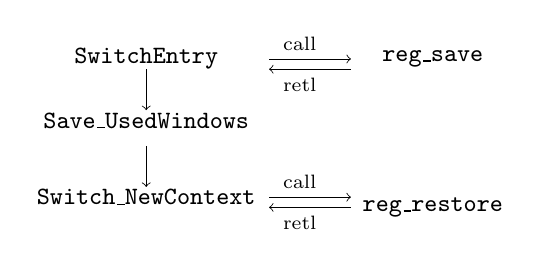
\begin{tikzpicture}[font=\small, line width=0.3pt, scale=1.3]
    \node(SwitchEntry) at (0, 2) {\texttt{SwitchEntry}};
    \node(call0) at (1.5, 2.15) {\scriptsize\text{call}};
    \draw[->] (1.2, 2) -- (2, 2);
    \node(retl0) at (1.5, 1.75) {\scriptsize\text{retl}};
    \draw[->] (2, 1.9) -- (1.2, 1.9);
    \draw[->] (0, 1.9) -- (0, 1.5);
    \node(regsave) at (2.8, 2) {\texttt{reg\_save}};

    \node(SaveUsedWindows) at (0, 1.4) {\texttt{Save\_UsedWindows}};
    \draw[->] (0, 1.15) -- (0, 0.75);

    \node(SwitchNewContext) at (0, 0.65) {\texttt{Switch\_NewContext}};
    \node(call1) at (1.5, 0.8) {\scriptsize\text{call}};
    \draw[->] (1.2, 0.65) -- (2, 0.65);
    \node(retl1) at (1.5, 0.4) {\scriptsize\text{retl}};
    \draw[->] (2, 0.55) -- (1.2, 0.55);
    \node(regrestore) at (2.8, 0.55) {\texttt{reg\_restore}};

    % \node(WindowOK) at (0, 1.4) {\texttt{Window\_OK}};
    % \draw[->] (-0.3, 1.25) -- (-1.6, 0.75);
    % \node(tcneqnull) at (-1.3, 1.2) {\tiny$t_c \neq \text{null}$};
    % \draw[->] (0.3, 1.25) -- (1.8, 0.5);
    % \node(tceqnull) at (1.3, 1.1) {\tiny$t_c = \text{null}$};

    % \node(regsave) at (-2, 0.6) {\texttt{reg\_save}};
    % \draw[->] (-2, 0.5) -- (-2, 0.1);
    % \node(SaveUsedWindows) at (-2, 0) {\texttt{Save\_UsedWindows}};
    % \draw[->] (-1.8, -0.15) -- (-0.5, -0.8);

    % \node(AdjustCWP) at (2, 0.3) {\texttt{Adjust\_CWP}};
    % \draw[->] (2, 0.2) -- (0.4, -0.8);
    % \node(SwitchNewContext) at (0, -0.9) {\texttt{Switch\_NewContext}};

    % \node(regrestore) at (2.8, -0.9) {\texttt{reg\_restore}};
    % \node(call) at (1.5, -0.7) {\tiny\text{call}};
    % \draw[->] (1.2, -0.85) -- (2, -0.85);
    % \node(retl) at (1.5, -1.1) {\tiny\text{retl}};
    % \draw[->] (2, -0.95) -- (1.2, -0.95);
\end{tikzpicture}
    \figurecaption{The Structure of Context Switch Routine}
	\label{fig:The Structure of Context Switch Routine}
\end{center}
\begin{itemize}
    \item \texttt{SwitchEntry}
    is the entry of the context switch routine.
    It saves the \localRN{} and \inRN{} registers of current
    window into the current task's stack in memory, and calls
    \texttt{reg\_save} to save other registers into 
    the current task's TCB.

    \item
    \texttt{Save\_UsedWindows} saves
	the register windows (except the current one)
    into the current task's stack in memory.
    % It checks whether the previous window is valid.
    % If yes, it uses the instruction $\crestore{}$
    % to set the previous window as the current one,
    % and saves its contents into stack (in memory),
    % then check the previous one continuously.

    \item
    \texttt{Switch\_NewContext}
    restores the general registers from the new task's TCB
    (by calling \texttt{reg\_restore})
    and its stack in memory
    respectively. Then it sets the new task as
    the current one.
\end{itemize}

The main complexity of the verification lies in
the code that manages the register window.
To save all the used
register windows, \texttt{Save\_UsedWindows}
repetitively restores the next window into general registers
(as the current window)
and then saves them into memory, until all the windows are saved.

\paragraph{\textbf{Specification.}}
Below we give the pre- and post-conditions
($\Apre$ and $\Apost$) of the verified module.
Each of them takes 6 arguments,
the id of the current task $\ctid$, the id of the new
task $\ntid$, the values $\env$ of general registers and
other register windows saving contexts,
the new task's context $\nst$ to be restored,
and the thread local state $\hthrdlocalst_c$
of current task and $\hthrdlocalst_n$ of the new task.
\[
    \small
    \begin{array}{l}
        \Apre(\ctid, \ntid, \env, \nst, \hthrdlocalst_c, \hthrdlocalst_n)
        \ \define \\
        \quad
        \begin{array}{l}
            \Env{\env} \sepstar
            (\relmsto{\TaskNew}{(\thrdid_n, 0)}) \sepstar
            \metricAst{10} \sepstar \\
            \quad
            \RelCurT{\thrdid_c}{\notCare}{\env}{\hthrdlocalst_c} \sepstar
            \RelRdyT{\thrdid_n}{\nst}{\hthrdlocalst_n} \sepstar
            \safePrimAst{\, \primsw(\nil) \,}
        \end{array}
        \\
        \\[-8pt]
        \Apost(\thrdid_c, \thrdid_n, \env, \nst, \hthrdlocalst_c, \hthrdlocalst_n)
        \ \define \\
        \quad
        \begin{array}{l}
            \exists \, \env', \hthrdlocalst'. \, \Env{\env'}
            \sepstar (\relmsto{\TaskNew}{(\thrdid_n, 0)})
            \sepstar \
            \\
            \quad
            (\RelCurT{\thrdid_n}{\nst}{\env'}{\hthrdlocalst'}
            \,\land\,\pEnv{\env'} = \nst) \sepstar
            \\
            \qquad
            \RelRdyT{\thrdid_c}{\pEnv{\env}}{\hthrdlocalst_c} \sepstar
            \safePrimAst{\, \primdone \,}
        \end{array}
    \end{array}
\]
In the specification,
we use $\Env{\env}$ to specify the values of
general registers and the register windows.
We describe the state
of the current task
% (its TCB and stack in memory)
using $\RelCurT{\ctid}{\notCare}{\env}{\hthrdlocalst_c}$.
It describes the memory of current task's TCB
and stack for saving contexts in low-level,
the thread local state $\hthrdlocalst_c$ in high-level,
and the state relation between the current thread $\ctid$
in low- and high-level.
Similarly, $\RelRdyT{\ntid}{\nst}{\hthrdlocalst_n}$
describes states of new task $\ntid$ in low- and high-level
programs and their relation.
% Here, we use $\nst$ to represent the saved context
% of task $\ntid$.
The memory location
$\TaskNew$ records the identifier of the new task $\ntid$.
And we use $\relmsto{\TaskNew}{(\ntid, 0)}$ to denote that
$\TaskNew$ saves $(\tid_n, 0)$
in both low- and high-level memory.
\[
    \relmsto{\loc}{\val} \ \define \
    (\msto{\loc}{\val}) \sepstar (\hmsto{\loc}{\val})
\]

The precondition takes ten tokens ($\metricAst{10}$).
As we have explained, verifying \call{}
and \jmp{} instructions will consume a token.
So, verifying the function calls
\regsave{} and \regrestore{} will
both consume a token. And \SaveUsedWin{},
which saves the context of each previous window
into memory repetitively until the invalid one,
% checks each previous window
% and saves its contexts into memory until the invalid one,
will execute at most eight times,
because the upper bound of
the number of windows is eight.
So, ten tokens is sufficient (two for \regsave{} and
\regrestore{}, and eight for \SaveUsedWin{}).

If we compare $\Apre$ and $\Apost$, we can see that
$\ntid$ becomes the current task
($\RelCurT{\ntid}{\nst}{\env'}{\hthrdlocalst'}$),
and its general registers and stack, specified by
$\Env{\env'}$, are loaded from the saved context
$\nst$ (\ie{} $\pEnv{\env'}\!=\!\nst$).
Here $\pEnv{\env'}$ refers to the part of the environment
that we want to save or restore as context.
Correspondingly, $\ctid$ becomes a non-current-thread,
and part of its environment $\env$ at the entry of
the context switch is saved, as specified by
$\RelRdyT{\ctid}{\pEnv{\env}}{\hthrdlocalst_c}$.
The execution of $\primsw$ should be done in the final state.
We use $\hthrdlocalst'$ to represent the thread local
state of $\ntid$ instead of $\hthrdlocalst_n$
in the final state, since the execution of
$\primsw$ will modify the program counters
in $\hthrdlocalst_n$.

\paragraph{\textbf{Proof outline}} We show how to use
our relational program logic defined in
\Fig{\ref{fig:Selected Inference Rules for Refinement Verification}}
to verify the correctness of the context switch routine.
We first instantiate the set of
abstract assembly primitives (\ref{ctxswitch-hprimset})
and the code heap specification (\ref{ctxswitch-Cspec})
below:
\begin{align}
    & \hprimset \ \define \ \{ \SwitchEntry \leadsto
        \primsw \}
        \label{ctxswitch-hprimset} \\
    & \!\begin{array}{lcl}
        \Cspec & \define &
        \{ \SwitchEntry \leadsto (\Apre, \Apost), \\
        & & \quad
        \regsave \leadsto
        (\relspecpre_{\textit{rs}}, \relspecpost_{\textit{rs}}),\\
        & & \quad
        \regrestore \leadsto
        (\relspecpre_{\textit{rr}}, \relspecpost_{\textit{rr}}) \\
        & & \quad
        \SaveUsedWin{} \leadsto (\relspecpre_{\textit{su}}, \relspecpost_{\textit{su}}), \\
        & & \quad
        \SwitchNewTask{} \leadsto (\relspecpre_{\textit{sn}}, \relspecpost_{\textit{sn}})
        \}
        \label{ctxswitch-Cspec}
    \end{array}
\end{align}

The set of abstract assembly primitive $\hprimset$
contains only one abstract assembly primitive $\primsw$.
And the code heap specification $\Cspec{}$
contains the specifications of each code block.
We use
$(\relspecpre_{\textit{rs}}, \relspecpost_{\textit{rs}})$,
$(\relspecpre_{\textit{rr}}, \relspecpost_{\textit{rr}})$,
$(\relspecpre_{\textit{su}}, \relspecpost_{\textit{su}})$ and
$(\relspecpre_{\textit{sn}}, \relspecpost_{\textit{sn}})$
to represent the specifications of
\regsave{}, \regrestore{},
\SaveUsedWin{} and \SwitchNewTask{} respectively.
Since the post-condition in our logic specifies the
state when the \textit{current function returns},
the specification of \SwitchEntry{} is $(\Apre, \Apost)$.
% We use
% $(\relspecpre_{\textit{rs}}, \relspecpost_{\textit{rs}})$,
% $(\relspecpre_{\textit{rr}}, \relspecpost_{\textit{rr}})$,
% $(\relspecpre_{\textit{su}}, \relspecpost_{\textit{su}})$ and
% $(\relspecpre_{\textit{sn}}, \relspecpost_{\textit{sn}})$ to
% represent the specifications of
% \regsave{}, \regrestore{},
% \SaveUsedWin{} and \SwitchNewTask{} respectively.

First, we prove that the specification of
context switch routine is well-defined in
Lemma~\ref{lemma:ctxswitch-wdspec}.
\begin{lemma}
    \em
    \label{lemma:ctxswitch-wdspec}
    $\wdSpec{\Apre}{\Apost}{\primsw}$
\end{lemma}
\begin{proof}
    By the definition of
    $\textsf{wdSpec}$ (defined in
    \Def{\ref{def:well-defined specification}}),
    we need to prove the following:
    % The correctness proof of this lemma is
    % straight-forward. According to the definition of
    % $\textsf{wdSpec}$ (defined in
    % \Def{\ref{def:well-defined specification}}),
    % we need to prove that the following three properties
    % hold:
    \begin{itemize}
        \item for any $\args{\val}, \hpstate, \hpstate', \hpstate_r$.
        if $\primsw(\args{\val})(\hpstate)(\hpstate')$, and
        $\hpstate \perp \hpstate_r$,
        then the following holds :
        \begin{itemize}
            \small
            \item $\hpstate'.\hthrdlocalst.\pc = \lab{} + 8$,
                $\hpstate'.\hthrdlocalst.\npc = \lab{} + 12$
                (where $\hpstate'.\hthrdlocalst.\hRstate.\hRfile
                    ({\reg{15}}) = \lab{}$);
            \item there exists $\hpstate'', \hpstate_r'$,
                $\primsw(\args{\val})(\hpstate \uplus \hpstate_r)
                    (\hpstate'')$, $\hpstate'' = \hpstate' \uplus \hpstate_r'$,
                and $\hpstate_r.\thrdpool = \hpstate_r'.\thrdpool$,
                $\hpstate_r.\Mem = \hpstate_r'.\Mem$;
        \end{itemize}

        Prove by the definition of $\primsw$, which
        ensures that, in the final state,
        the program counters will point to
        the correct pointers and the threads and
        memory in $\hpstate_r$ remain unchanged,
        because the execution of $\primsw$ only accesses
        the current and new tasks in thread pool
        and the location $\TaskNew$ in memory.

        % The definition of $\primsw$ ensures that the
        % program counters will point to the correct pointers,
        % and its execution only accesses
        % the current and new tasks in thread pool
        % and the location $\TaskNew$ in memory.
        % So, the threads and memory specified in $\hpstate_r$
        % remain unchanged in final state.

        \item for any $\thrdid_c, \thrdid_n, \env, \nst, \hthrdlocalst_c, \hthrdlocalst_n$,
            \begin{itemize}
                \small
                \item $\Apre(\thrdid_c, \thrdid_n, \env, \nst, \hthrdlocalst_c, \hthrdlocalst_n)
                    \Rightarrow \safePrimAst{\primsw} \sepstar \atrue$;
                \item $\Apost(\thrdid_c, \thrdid_n, \env, \nst, \hthrdlocalst_c, \hthrdlocalst_n)
                    \Rightarrow \safePrimAst{\primdone} \sepstar \atrue$;
            \end{itemize}
        \vspace*{0.3em}
        Prove by the definition of $\Apre$ and $\Apost$.
        % According the definition of $\Apre$ and $\Apost$,
        % we are done.

        \item for any $\args{\val}, \state, \hpstate$,
        if $(\state, \hpstate, \notCare, \notCare) \in
            \INV{(\primsw(\args{\val}), \args{\val})}$,
        then there exists $\thrdid_c, \thrdid_n, \env$, $\nst,
        \hthrdlocalst_c, \hthrdlocalst_n, \relastP_r$ and $\word$,
        such that:
        \begin{itemize}
            \small
            \item $\asrtmodel{(\state, \hpstate, \primsw(\args{\val}), \word)}
                {\Apre(\thrdid_c, \thrdid_n, \env, \nst, \hthrdlocalst_c,
                \hthrdlocalst_n) \sepstar \relastP_r}$;
            \item  $(\Apost(\thrdid_c, \thrdid_n, \env, \nst, \hthrdlocalst_c,
                \hthrdlocalst_n) \sepstar \relastP_r) \Rightarrow
                \INV{(\primdone, \notCare)}$;
            \item $\Sta(\primsw(\args{\val}), \relastP_r)$.
        \end{itemize}

        Prove by the definitions of $\Apre$ and $\Apost$.
        They specify the states of task $\tid_c$ and
        $\tid_n$ and memory location $\TaskNew$
        % of original current task $\tid_c$,
        % new task $\tid_n$ and memory location $\TaskNew$
        in low- and high-level. And we define the frame
        % The definitions of $\Apre$ and $\Apost$ describe that
        % the states of original current task $\tid_c$,
        % new task $\tid_n$ and memory location $\TaskNew$
        % in low- and high-level.
        % We define the frame
        $\relastP_r$ to depict the state of the
        remaining tasks and memory
        (excluding tasks $\tid_c$, $\tid_n$, and
        memory location $\TaskNew$) in low- and high-level.
        Then, we can prove that the
        state relation between low- and high-level
        holds at the entry and
        exit of the context switch routine.
        Since the execution of $\primsw$ only accesses
        the current and new tasks in thread pool, and the
        memory location $\TaskNew$,
        the threads and memory specified in assertion
        $\relastP_r$ remain unchanged
        in the final state and $\relastP_r$ keeps
        stable ($\Sta(\primsw, \relastP_r)$).
    \end{itemize}
    % Thus we are done.
\end{proof}

We use $\code_{\texttt{switch}}$ to represent the
code heap storing the code of context switch routine,
which includes the code blocks \SwitchEntry{},
\regsave{}, \regrestore{},
\SaveUsedWin{} and \SwitchNewTask{}. We prove that
the $\code_{\texttt{switch}}$ is well-defined in
Lemma~\ref{lemma:ctxswitch-wfcdhp}.

\begin{lemma}
    \em
    \label{lemma:ctxswitch-wfcdhp}
    $\wfcdhp{\code_{\texttt{switch}}}{\Cspec{}}$
\end{lemma}
\begin{proof}
    The code heap specification $\Cspec{}$ have been
    defined in (\ref{ctxswitch-Cspec}). We unfold
    $\wfcdhp{\code_{\texttt{switch}}}{\Cspec{}}$
    according to its definition
    (in \Fig{\ref{fig:Selected Inference Rules for Refinement Verification}}).
    And we need to prove that for any $\lgvl_1$,
    $\lgvl_2$, $\lgvl_3$,
    $\lgvl_4$ and $\lgvl_5$, the following hold
    (we use $\lab{\textit{se}}$, $\lab{\textit{rs}}$,
    $\lab{\textit{rr}}$, $\lab{\textit{su}}$ and
    $\lab{\textit{sn}}$ to represent the starting labels of
    \SwitchEntry{}, \regsave{}, \regrestore{},
    \SaveUsedWin{} and \SwitchNewTask{} below):
    \begin{align}
        & \wfcblk{\Apre \ \lgvl_1}{\Apost \ \lgvl_1}
            {\lab{\textit{se}}}
            {\code_{\texttt{switch}}
            [\lab{\textit{se}}]}
            \tag{g-wfse}
            \label{ctxswitch-wfse} \\
        & \wfcblk{\relspecpre_{\textit{rs}} \ \lgvl_2}
            {\relspecpost_{\textit{rs}} \ \lgvl_2}
            {\lab{\textit{rs}}}
            {\code_{\texttt{switch}}
            [\lab{\textit{rs}}]}
            \tag{g-wfrs}
            \label{ctxswitch-wfrs} \\
        & \wfcblk{\relspecpre_{\textit{rr}} \ \lgvl_3}
            {\relspecpost_{\textit{rr}}\ \lgvl_3}
            {\lab{\textit{rr}}}
            {\code_{\texttt{switch}}
            [\lab{\textit{rr}}]}
            \tag{g-wfrr}
            \label{ctxswitch-wfrr} \\
        & \wfcblk{\relspecpre_{\textit{su}} \ \lgvl_4}
            {\relspecpost_{\textit{su}} \ \lgvl_4}
            {\lab{\textit{su}}}
            {\code_{\texttt{switch}}[\lab{\textit{su}}]}
            \tag{g-wfsu}
            \label{ctxswitch-wfsu} \\
        & \wfcblk{\relspecpre_{\textit{sn}} \ \lgvl_5}
            {\relspecpost_{\textit{sn}} \ \lgvl_5}
            {\lab{\textit{sn}}}
            {\code_{\texttt{switch}}[\lab{\textit{sn}}]}
            \tag{g-wfsn}
            \label{ctxswitch-wfsn}
    \end{align}

    \begin{center}
        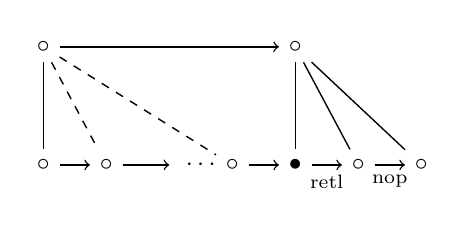
\begin{tikzpicture}[font=\small, line width=0.5pt]
    \node(S1) at (0, 1.5) {$\circ$};
    \node(S2) at (3.2, 1.5) {$\circ$};

    %%%%%%%%%%%%%%%%%%%%%%%%%%%%%%%%%%%%%%%%%%%%%%
    \node(T1) at (0, 0) {$\circ$};
    \node(T2) at (0.8, 0) {$\circ$};
    \node(T3) at (2.4, 0) {$\circ$};
    \node(T4) at (3.2, 0) {$\bullet$};
    \node(T5) at (4, 0) {$\circ$};
    \node(T6) at (4.8, 0) {$\circ$};

    %%%%%%%%%%%%%%%%%%%%%%%%%%%%%%%%%%%%%%%%%%%%%%
    \draw[-] (S1) to (T1);
    \draw[-, dashed] (S1) to (T2);
    \draw[-, dashed] (S1) to (T3);
    \draw[-] (S2) to (T4);
    \draw[-] (S2) to (T5);
    \draw[-] (S2) to (T6);

    \draw[->] (S1) to node[above]{\scriptsize $\primsw{}$} (S2);

    \draw[->] (T1) to (T2);
    \draw[->] (T2) to (1.6, 0);
    \node(dots) at (2, 0) {$\cdots$};
    \draw[->] (T3) to (T4);
    \draw[->] (T4) to node[below]{\scriptsize retl} (T5);
    \draw[->] (T5) to node[below]{\scriptsize nop} (T6);

    % \node(hexec) at (3.2, -1) 
    %     {\scriptsize
    %     $\begin{array}{l}
    %         \text{apply } \myrule{ABSCSQ} \\
    %         \text{rule}
    %     \end{array}$};
\end{tikzpicture}
        \vspace*{-0.5em}
        \figurecaption{Point doing refinement reasoning}
        \label{fig:refinement reasoning}
    \end{center}

    The correctness proof from
    (\ref{ctxswitch-wfse}) to (\ref{ctxswitch-wfsn})
    can be done by applying the inference rules for
    code block shown in
    \Fig{\ref{fig:Selected Inference Rules for Refinement Verification}}.
    We can choose any place to apply
    \myrule{ABSCSQ} rule to execute primitive $\primsw$.
    Here, we apply \myrule{ABSCSQ} rule
    in verifying the code block
    \SwitchNewTask{} (\ref{ctxswitch-wfsn}),
    when context switch routine returns,
    as shown in \Fig{\ref{fig:refinement reasoning}}.
    In \Fig{\ref{fig:refinement reasoning}}, we use the
    solid circle to represent the point applying \myrule{ABSCSQ} rule,
    and after the execution of $\primsw$, the
    state relation between low- and high-level can
    be reestablished and we use solid line to represent
    that such relation holds in \Fig{\ref{fig:refinement reasoning}}.
    % and prove that the state
    % relation between low- and high-level programs
    % can be reestablished in verifying
    % (\ref{ctxswitch-wfsn}), when context switch routine
    % returns, as shown in \Fig{\ref{fig:refinement reasoning}}.
    % In \Fig{\ref{fig:refinement reasoning}}, we use the
    % solid circle to represent the point applying \myrule{ABSCSQ} rule,
    % and use the solid line to repesent that
    % the state relation
    % between low- and high-level holds.
\end{proof}

\begin{theorem}[Context Switch Routine Correctness]
    \em
    $\wfprim{\Cspec}{\code_{\texttt{switch}}}{\hprimset}$.
\end{theorem}
\begin{proof}
    By the definition of
    $\wfprim{\Cspec}{\code_{\texttt{switch}}}{\hprimset}$,
    where $\hprimset$ and $\Cspec{}$ are defined in
    (\ref{ctxswitch-hprimset}) and (\ref{ctxswitch-Cspec})
    respectively, we prove the following:
    % We unfold
    % $\wfprim{\Cspec}{\code_{\texttt{switch}}}{\hprimset}$
    % by its definition
    % (in \Fig{\ref{fig:Selected Inference Rules for Refinement Verification}}),
    % where $\hprimset$ and $\Cspec{}$ are defined in
    % (\ref{ctxswitch-hprimset}) and (\ref{ctxswitch-Cspec})
    % respectively, and we prove the following hold:
    \begin{itemize}
        \item $\wfcdhp{\asmimp}{\Cspec{}}$.
            Prove by applying Lemma~\ref{lemma:ctxswitch-wfcdhp}.
            % The correctness proof of this subgoal can be done by
            % apply Lemma~\ref{lemma:ctxswitch-wfcdhp}.
        \item $\wdSpec{\Apre}{\apost}{\primsw}$.
            Prove by applying Lemma ~\ref{lemma:ctxswitch-wdspec}.
            % The correctness proof of this subgoal can be done by
            % apply Lemma~\ref{lemma:ctxswitch-wdspec}.
    \end{itemize}
    % Thus we are done.
\end{proof}

This part of work has not been mechanized in Coq.
In our conference paper, we show that
we apply our logic that do not support
refinement verification to verify
the main body of the context switch routine in
a realistic embedded OS kernel for aerospace crafts,
which consists of around 250 lines of SPARCv8 code,
by 6690 lines of Coq proof scripts. Here, the
context switch routine verified by applying our
relational program logic is a
simplified version of such context switch routine,
which omits some details like judging whether the
current thread is a valid thread.
Verifying that each code block is well-defined
by applying the inference rules in our new logic is
no different from the previous proof work.
The additional proof efforts include:
(1) proving that the specification of context
switch routine is well-defined (presented in
Lemma~\ref{lemma:ctxswitch-wdspec});
(2) applying \myrule{ABSCSQ} rule to execute
the $\primsw$ primitive and proving that the state
relation between low- and high-level programs
can be reestablished in verifying code block
\SwitchNewTask{}, when the context switch routine
returns (as noted in the proof of
Lemma~\ref{lemma:ctxswitch-wfcdhp}).

% We present more details of this part of proof
% work in TR~\cite{coqimp}.
We present more details of proof in TR~\cite{coqimp}.